\documentclass[12pt, letterpaper]{article}
\usepackage[top=2.5cm, bottom=2.5cm, left=3cm, right=2.5cm]{geometry}
\usepackage[utf8]{inputenc}
\usepackage[T1]{fontenc}
\usepackage{lmodern}
\usepackage{amsmath, amssymb}
\usepackage{booktabs}
\usepackage{tabularx}
\usepackage{longtable}
\usepackage{array}
\usepackage{multirow}
\usepackage{xcolor}
\usepackage{graphicx}
\usepackage{float}
\usepackage{listings}
\usepackage[most, breakable]{tcolorbox}
\usepackage{enumitem}
\usepackage{fancyhdr}
\usepackage{titlesec}
\usepackage{setspace}
\usepackage{microtype}
\usepackage[hidelinks]{hyperref}
\usepackage{parskip}
\usepackage{pgfplots}
\pgfplotsset{compat=1.15}
\usepackage{tikz}
\usepackage{subcaption}

% Optional clean color definitions (replace if you already have them)
\definecolor{beteal}{RGB}{0,128,128}
\definecolor{berust}{RGB}{180,60,60}
\definecolor{beblue}{RGB}{50,90,180}
\definecolor{bepurple}{RGB}{120,60,160}

% Define colors (replace if already defined in your preamble)
\usepackage{xcolor}
\definecolor{berust}{RGB}{180,60,60}
\definecolor{beteal}{RGB}{0,140,140}
% Colours
\definecolor{econblue}{RGB}{31,78,121}
\definecolor{researchgreen}{RGB}{21,101,45}
\definecolor{exampleorange}{RGB}{180,80,20}
\definecolor{lightgray}{RGB}{245,245,245}
\definecolor{boxblue}{RGB}{220,235,248}

% Section headings
\titleformat{\section}{\large\bfseries\color{econblue}}{\thesection}{1em}{}%
  [\vspace{-4pt}\rule{\linewidth}{0.4pt}]
\titleformat{\subsection}{\normalsize\bfseries\color{econblue}}{\thesubsection}{1em}{}
\titleformat{\subsubsection}{\normalsize\bfseries}{\thesubsubsection}{1em}{}

% Page style
\pagestyle{fancy}
\fancyhf{}
\fancyhead[L]{\small\itshape ECON 230 --- Introduction to Behavioural Economics}
\fancyhead[R]{\small\itshape Chapter 6: More Than Money}
\fancyfoot[C]{\small\thepage}
\renewcommand{\headrulewidth}{0.4pt}
\setlength{\headheight}{14pt}

% tcolorbox styles
\tcbuselibrary{breakable, skins, listings}

\newtcolorbox{researchbox}{
  enhanced, breakable,
  colback=researchgreen!6, colframe=researchgreen!55,
  title=\textbf{Research Study},
  fonttitle=\bfseries\small,
  attach boxed title to top left={yshift=-2mm, xshift=6mm},
  boxed title style={colback=researchgreen!55, colframe=researchgreen!55},
  before upper={\setlength{\parskip}{4pt}}
}

\newtcolorbox{examplebox}[1]{
  enhanced, breakable,
  colback=exampleorange!6, colframe=exampleorange!45,
  title=\textbf{#1}, fonttitle=\bfseries\small
}

\newtcolorbox{keybox}{
  enhanced, colback=boxblue, colframe=econblue!70,
  fontupper=\small
}

% ASCII figure style
\lstset{
  basicstyle=\scriptsize\ttfamily,
  breaklines=false,
  keepspaces=true,
  columns=flexible,
  frame=single,
  backgroundcolor=\color{lightgray},
  xleftmargin=4pt, xrightmargin=4pt,
  aboveskip=6pt, belowskip=6pt
}

% Lists
\setlist[itemize]{leftmargin=1.5em, itemsep=2pt, topsep=4pt}
\setlist[enumerate]{leftmargin=1.5em, itemsep=2pt, topsep=4pt}
\onehalfspacing

\newcolumntype{Y}{>{\raggedright\arraybackslash}X}

\begin{document}

\begin{titlepage}
\centering\vspace*{3cm}
{\Large\bfseries\color{econblue} ECON 230 --- Introduction to Behavioural Economics\\[1em]}
{\large\bfseries Course Textbook\\[2em]}
{\LARGE\bfseries\color{econblue} Chapter 6\\[0.5em]}
{\Large\bfseries More Than Money --- Social Preferences, Fairness, and Reciprocity\\[2em]}
\vfill
{\normalsize University of Northern British Columbia\\
Instructor: Prof.\ Muhebullah Karimzada\\
Term: Winter 2027}
\end{titlepage}
\tableofcontents
\newpage


\medskip


\section*{Chapter Overview}
\addcontentsline{toc}{section}{Chapter Overview}


The first five chapters of this textbook examined how individuals make decisions involving risk, uncertainty, time, and their own financial resources. In every case, the implicit model was that of an isolated agent choosing from a menu of options that affect only their own wellbeing. This simplification was useful for building the foundational tools of behavioural economics --- Prospect Theory, the $\beta$-$\delta$ model, mental accounting --- but it leaves out something essential about human decision-making. Most economically important decisions take place in social contexts: with partners, employers, employees, neighbours, governments, and strangers. And in social contexts, people's motivations turn out to be dramatically richer than the pure self-interest standard model assumes.

This chapter documents and analyses \textbf{social preferences}: genuine concerns about others' outcomes, about fairness, about reciprocity, and about social norms that extend well beyond own-payoff maximisation. The evidence comes from a remarkably clean and replicable set of experimental designs --- the ultimatum game, the dictator game, the trust game, and the public goods game --- that have been conducted in dozens of countries across five decades, consistently producing results that the standard model cannot explain.

We then turn to formal models. The \textbf{Fehr-Schmidt model} (1999) provides an elegant quantitative framework: agents experience disutility both from having less than others (disadvantageous inequality, or envy) and from having more than others (advantageous inequality, or guilt). We examine the model's predictions, its successes, and its limitations. We also discuss reciprocity-based approaches, which emphasise that people respond to perceived intentions --- not just payoff distributions --- and pure altruism, where giving reflects genuine concern for others' welfare.

The applications section shows why social preferences matter economically: they help explain efficiency wages, wage rigidity, the persistence of corruption norms, the functioning of labour markets, the basis of trust as productive social capital, and the challenges of designing effective incentive systems. Social preferences are not peripheral psychological curiosities --- they are central to how economies actually function.

\medskip


\section*{Learning Objectives}
\addcontentsline{toc}{section}{Learning Objectives}


After studying this chapter, students should be able to:

\begin{enumerate}
\item \textbf{Define} social preferences and explain why the standard self-interest model fails to account for them.
\item \textbf{Describe} the ultimatum game and interpret the typical empirical findings, including the rejection of positive offers.
\item \textbf{Explain} what the dictator game isolates and what the typical giving pattern reveals about motives for generosity.
\item \textbf{Describe} the trust game and interpret the results in terms of trust, trustworthiness, and social capital.
\item \textbf{Define} the Fehr-Schmidt model of inequality aversion, state the utility function, interpret the parameters $\alpha$ and $\beta$, and use the model to predict behaviour in the ultimatum game.
\item \textbf{Distinguish} between disadvantageous inequality aversion (envy), advantageous inequality aversion (guilt), altruism, and reciprocity as distinct social preference motivations.
\item \textbf{Explain} altruistic punishment and the public goods game evidence from Fehr and Gächter (2002), including what happens to cooperation with and without punishment.
\item \textbf{Define} warm glow altruism and explain how it differs from pure altruism.
\item \textbf{Apply} social preference theory to labour market phenomena, including efficiency wages, gift exchange, and wage rigidity.
\item \textbf{Evaluate} the evidence on social trust as a determinant of economic performance and interpret findings on the persistence of corruption norms.
\end{enumerate}

\newpage


\section*{Introduction: Would You Sacrifice Money to Punish Unfairness?}
\addcontentsline{toc}{section}{Introduction: Would You Sacrifice Money to Punish Unfairness?}


You and a stranger have been given \$30 to divide. The stranger decides how to split it. They offer you \$5, keeping \$25 for themselves. You have two options: accept the \$5, or reject --- in which case you both receive nothing.

Standard economics says the answer is obvious: accept. Five dollars is more than zero dollars, and your preferences should be defined over your own payoff. What the stranger keeps is irrelevant to you.

Yet in hundreds of experiments conducted across the world, approximately 50\% of people in this situation reject offers below \$3 out of \$10. They sacrifice a real payoff --- real money, real goods --- to punish someone they judge to have behaved unfairly. They do this even when the interaction is anonymous and will never be repeated. They do this even when the stakes are raised to several months' salary. They do this in developed and developing economies alike, across cultures and age groups.

This behaviour cannot be explained by self-interest. But it is not random noise, either. It is systematic, stable across replications, and deeply connected to a set of human motivations that standard economics has largely set aside: concerns about fairness, about being treated with respect, about what others receive relative to oneself, and about the social consequences of allowing violations of norms to go unpunished.

These motivations are what this chapter calls \textbf{social preferences}. They are not exotic exceptions to the rule of self-interest --- they are pervasive features of human economic life, with large consequences for markets, organisations, and public policy. Understanding them is the subject of this chapter.

\newpage


\section{The Standard Model and Its Failures}



\subsection{The Self-Interest Assumption}


Standard economics makes a stark and useful assumption: agents care only about their own material payoffs. More precisely, the utility of agent $i$ depends only on $i$'s own consumption or payoff $x_i$:

$$U_i = u_i(x_i)$$

Other agents' payoffs enter agent $i$'s utility only indirectly --- through prices, competition, public goods, or externalities --- not directly. If a complete stranger receives \$1,000, this has no direct effect on agent $i$'s utility, so long as it doesn't affect any price or constraint that $i$ faces.

This assumption generates powerful results. In competitive markets with large numbers of agents, self-interest generates efficient outcomes through the price system. In game theory, self-interest underpins the concept of Nash equilibrium --- the prediction that each player will choose the strategy that maximises their own payoff given what others are doing.

The self-interest assumption is useful not because economists believe it is literally true --- Adam Smith, often misread as its proponent, wrote extensively about human sympathy and moral sentiments in his 1759 \textit{Theory of Moral Sentiments} --- but because it generates sharp, testable predictions. Those predictions have now been tested extensively in carefully controlled experiments, and the results are clear: the self-interest model systematically underestimates how much people care about others.


\subsection{The Experimental Evidence: A Preview}


Four experimental paradigms have generated the bulk of the evidence against pure self-interest. Each isolates a different dimension of social motivation. Their results are summarised in the table below before being examined in detail.
\newpage
\textbf{Table 6.1: Standard Economics Predictions versus Experimental Evidence}


\begin{table}[H]
\centering
\small
\begin{tabularx}{\linewidth}{lYY}
\toprule
Experiment & Standard (Nash) Prediction & Typical Experimental Result \\
\midrule
\textbf{Ultimatum Game} & Proposer offers minimum possible (\$0.01); Responder accepts anything > 0 & Mean offer $\approx$ 40--44\% of pie; 40--60\% reject offers below 20\% \\
\textbf{Dictator Game} & Give \$0 (no strategic motive for giving) & Mean giving $\approx$ 28\% of endowment; only 36\% give \$0 \\
\textbf{Trust Game} & Investor sends \$0 (anticipating trustee returns nothing) & Average sent $\approx$ 50\%; average return $\approx$ 37\% of tripled amount \\
\textbf{Public Goods Game} & Contribute \$0 (dominant strategy is free-ride) & Initial contributions 40--60\%; declines without punishment mechanism \\
\bottomrule
\end{tabularx}
\end{table}


In every case, the standard model's prediction is at the extreme end of what rational self-interest implies --- and the actual behaviour is substantially further from that extreme. The gap is not noise. It has been replicated thousands of times across dozens of countries, across different stake sizes, different demographic groups, and different institutional contexts.

\medskip


\section{The Ultimatum Game}



\subsection{The Design}


The ultimatum game is the simplest and most widely studied experiment in behavioural economics. Two players --- typically called the Proposer and the Responder --- interact over a fixed sum of money (the "pie"). The Proposer decides how to split the pie, naming an offer for the Responder. The Responder then either \textbf{accepts} (both players receive their allotted shares) or \textbf{rejects} (both players receive nothing).

The game is called "ultimatum" because the Proposer makes a single take-it-or-leave-it offer with no negotiation. It has a unique subgame perfect Nash equilibrium under the self-interest assumption: the Proposer offers the smallest possible positive amount (say, one cent), and the Responder accepts, because one cent is more than zero and a rational self-interested Responder prefers any positive amount to nothing.

\newpage
\subsection{The Evidence}


The evidence deviates dramatically from this prediction in two directions simultaneously:

\textbf{Proposers offer too much.} Rather than offering the minimum, the overwhelming majority of Proposers in ultimatum experiments offer between 40\% and 50\% of the pie. Very few offer less than 20\%. In a meta-analysis of 37 studies covering more than 75,000 observations, Oosterbeek, Sloof, and van de Kuilen (2004) found a mean offer of approximately 40--44\% of the pie across cultures.

\textbf{Responders reject positive offers.} Rather than accepting any positive offer, Responders frequently reject offers they perceive as unfair. The rejection rate for offers of approximately 20\% or less (one-fifth of the pie) ranges from 40--60\% across studies. Offers below 10\% are rejected by approximately 75--90\% of Responders. The rejection rate falls sharply as the offer rises, approaching zero for offers near 50\%.

\textbf{High-stakes replications.} A standard objection to laboratory experiments is that the stakes are trivial --- perhaps people reject \$1 out of a \$5 pie just to make a point, but they would not reject \$1,000 out of a \$5,000 pie. This objection has been tested directly. Slonim and Roth (1998) ran ultimatum experiments in Slovakia with stakes equivalent to a month's salary; Cameron (1999) ran them in Indonesia with stakes equivalent to three months' average income. In both cases, the qualitative pattern --- significant rejection of low offers --- persisted. Higher stakes reduced rejections marginally (as predicted by rational models in which the value of the signal is fixed relative to a larger payoff), but did not eliminate them.

The conclusion: rejection of low offers in the ultimatum game is not a laboratory artefact produced by low stakes or lack of engagement. It reflects genuine preferences that people bring to economic interactions.

\newpage
\textbf{Figure 6.1: The Ultimatum Rejection Curve}

\begin{figure}[h!]
\centering

\begin{tikzpicture}
\begin{axis}[
  width=0.8\textwidth,
  height=0.5\textheight,
  xlabel={Offer (\% of pie)},
  ylabel={Rejection Rate (\%)},
  xmin=0, xmax=50,
  ymin=0, ymax=100,
  axis lines=left,
  grid=both,
  title={Ultimatum Rejection Curve (Meta-analysis)},
  legend style={font=\small, at={(0.97,0.95)}, anchor=north east},
  tick label style={font=\small},
  label style={font=\small},
  title style={font=\small},
]

% Main rejection curve
\addplot[
  very thick,
  color=berust,
  mark=*,
  mark size=1.5pt
] coordinates {
  (5,90)(10,75)(15,55)(20,35)(25,18)
  (30,8)(35,3)(40,1)(45,0)(50,0)
};
\addlegendentry{Rejection rate}

% Nash benchmark line
\addplot[
  dashed,
  thick,
  color=beteal
] coordinates {(0,0)(50,0)};
\addlegendentry{Nash: accept all}

% Label for Nash line (placed away from overlap)
\node[font=\small, text=beteal] at (axis cs:42,6) {Nash prediction};

\end{axis}
\end{tikzpicture}

\caption{Experimental evidence from ultimatum games: rejection rates fall sharply as offers increase, consistent with fairness-driven thresholds rather than purely monetary acceptance.}
\end{figure}



\begin{table}[H]
\centering
\small
\begin{tabularx}{\linewidth}{lY}
\toprule
 & Description \\
\midrule
\textbf{What the figure shows} & A downward-sloping curve plotting the rejection rate (vertical axis, 0--100\%) against the offer as a percentage of the pie (horizontal axis, 0--50\%). The rejection rate is approximately 90\% at an offer of 5\%, falls to about 55\% at 15\%, 35\% at 20\%, 18\% at 25\%, and approaches zero for offers above 35\%. A flat horizontal line at 0\% represents the Nash equilibrium prediction (accept everything). \\
\textbf{How to interpret it} & Every point above the horizontal axis represents a systematic departure from the Nash equilibrium prediction. The steep negative slope shows that rejection is highly sensitive to the offer level, consistent with a threshold of acceptable fairness that varies across individuals. \\
\bottomrule
\end{tabularx}
\end{table}





\subsection{Cross-Cultural Evidence}


A particularly important question is whether the preference for fair treatment is universal or culturally specific. The most ambitious cross-cultural study was conducted by Henrich and colleagues (2001, 2004), who ran ultimatum games in 15 small-scale societies across Africa, Asia, Oceania, and the Americas, including hunter-gatherers, horticulturalists, and pastoralists.

The findings were remarkable in two respects. First, \textbf{no society came close to the Nash equilibrium prediction.} Even in the society with the lowest mean offer --- the Machiguenga of Peru, who offered on average 26\% --- the behaviour was substantially above the Nash prediction, and rejection was rare but not absent. Second, the \textbf{variation across societies was substantial and systematic}: mean offers ranged from 26\% (Machiguenga) to 57\% (Lamelara of Indonesia).

Critically, the variation across societies was predicted by the societies' economic structures and cultural norms around resource sharing. The Lamelara, who engage in cooperative whale hunting and have strong norms of resource sharing, made hyper-fair offers --- and some responders \textit{rejected} these as embarrassingly generous (an "over-generous" offer violates social norms in the opposite direction from unfair ones). The Machiguenga, who live in highly atomistic nuclear families with little community-level economic coordination, made lower offers and showed low rejection rates --- consistent with weaker norms of interpersonal fairness in market transactions.
\newpage
\begin{researchbox}
\textbf{Research Study: In Search of Homo Economicus --- Ultimatum Games in 15 Societies}\\[4pt]

\textbf{Researchers:} Joseph Henrich, Robert Boyd, Samuel Bowles, Colin Camerer, Ernst Fehr, Herbert Gintis, and Richard McElreath\\[4pt]
\textbf{Year:} 2001 (first paper); expanded in 2004\\[4pt]
\textbf{Research Question:} Are the social preferences documented in ultimatum games in Western economies universal features of human motivation, or culturally specific products of Western market economies?\\[4pt]
\textbf{Method:} Researchers ran ultimatum games with substantial stakes (local goods worth meaningful amounts relative to local income) in 15 small-scale societies that varied widely in their economic organisation, market integration, and cultural norms around sharing and fairness.\\[4pt]
\textbf{Results:} Mean offers ranged from 26\% (Machiguenga) to 57\% (Lamelara). No society produced offers near the Nash equilibrium prediction. Rejection patterns varied significantly: some societies showed low rejection even of low offers (Machiguenga), while others showed rejection of both very low and very high offers (Lamelara).\\[4pt]
\textbf{Economic Interpretation:} The universality of departure from self-interest --- combined with the systematic variation in the form that departure takes --- suggests that social preferences are a genuine feature of human psychology, but that their specific content is shaped by the economic and cultural institutions within which people live. Market integration, in particular, was positively associated with higher offers and stronger rejection of unfair treatment.\\[4pt]
\textbf{Behavioural Insight:} The finding that market integration correlates with fairer ultimatum offers is striking: exposure to impersonal market exchange, far from making people more selfish, appears to build norms of fairness and respect for trading partners. Pure self-interest in market exchange requires enforcement mechanisms that impersonal markets must substitute for personal relationship-based trust.\\[4pt]
\end{researchbox}

\medskip


\section{The Dictator Game}



\subsection{Separating Fairness from Strategy}


The ultimatum game documents both the preference for fair treatment and the willingness to punish unfairness. But it cannot cleanly separate these motivations: the Proposer may offer 40\% not because they care about fairness but because they fear rejection. The Responder rejects not just because of fairness preferences but also to punish the Proposer.

The \textbf{dictator game} eliminates strategic considerations entirely. The setup is identical to the ultimatum game except that the Responder has no choice --- they must accept whatever the Dictator offers. Any giving by the Dictator is therefore a \textbf{pure expression of social preference}: there is no fear of rejection, no strategic motive, no reputation to maintain (experiments are typically anonymous). Whatever the Dictator gives, they give because they genuinely prefer a less unequal distribution.


\subsection{The Evidence}


The standard economic prediction in the dictator game is unambiguous: a self-interested Dictator will give nothing, keeping the entire endowment.

The evidence again strongly contradicts this. Engel (2011) conducted a meta-analysis of 616 dictator game studies encompassing more than 20,000 observations. The findings:

\begin{itemize}
\item \textbf{Mean giving: 28.3\%} of the endowment. Dictators give away more than a quarter of their money to strangers, on average, with no strategic reason to do so.
\item \textbf{36\% give \$0:} The largest single category is those who give nothing --- consistent with pure self-interest --- but this is less than half the population.
\item \textbf{17\% give exactly 50\%:} The modal "generous" choice is an exactly equal split, consistent with a strong norm of equality in the absence of strategic concerns.
\item Giving is distributed across all amounts, with peaks at \$0 and at \$5 (the equal split), and declining frequency at intermediate amounts.
\end{itemize}
\newpage
\textbf{Figure 6.2: Dictator Game Giving Distribution}


\begin{figure}[ht]
\centering
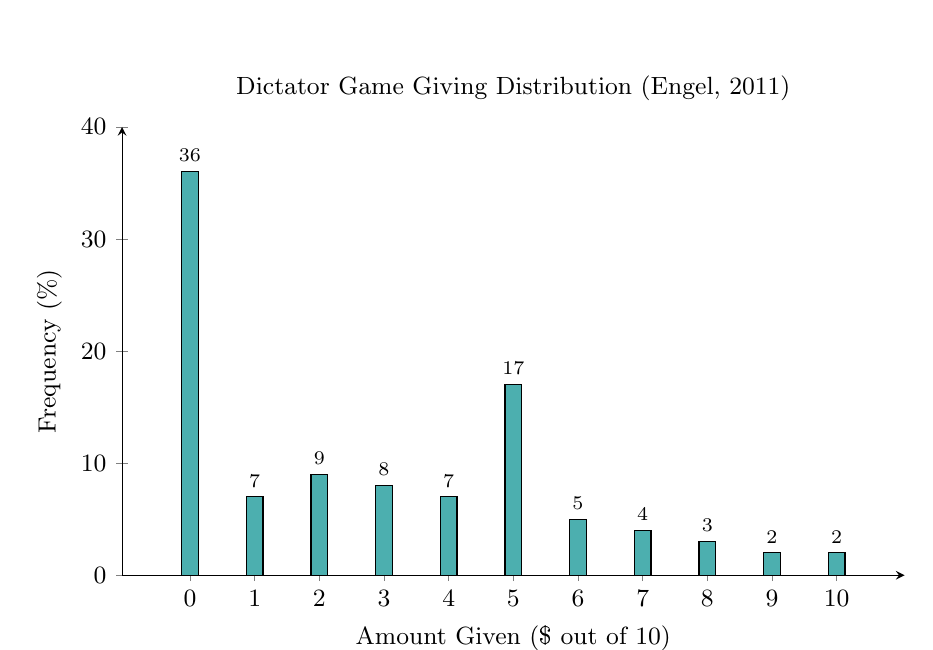
\begin{tikzpicture}
\begin{axis}[
    width=0.95\textwidth,
    height=0.6\textwidth,
    ybar,
    bar width=6pt,
    ymin=0, ymax=40,
    xmin=-0.5, xmax=10.5,
    xtick={0,1,...,10},
    xlabel={Amount Given (\$ out of 10)},
    ylabel={Frequency (\%)},
    title={Dictator Game Giving Distribution (Engel, 2011)},
    axis lines=left,
    enlarge x limits=0.05,
    tick label style={font=\small},
    label style={font=\small},
    title style={font=\small},
    nodes near coords,
    nodes near coords align={vertical},
    every node near coord/.append style={font=\scriptsize},
]

\addplot[
    fill=beteal!70,
    draw=black,
] coordinates {
    (0,36)
    (1,7)
    (2,9)
    (3,8)
    (4,7)
    (5,17)
    (6,5)
    (7,4)
    (8,3)
    (9,2)
    (10,2)
};

\end{axis}
\end{tikzpicture}
\caption{Distribution of giving in the dictator game. Data from Engel (2011).}
\end{figure}


\begin{table}[H]
\centering
\small
\begin{tabularx}{\linewidth}{lY}
\toprule
 & Description \\
\midrule
\textbf{What the figure shows} & A bar chart showing the distribution of dictator game offers from a meta-analysis of 616 papers (Engel, 2011). The horizontal axis shows the amount given (0 to 10, as fractions of a \$10 endowment). The vertical axis shows the percentage of dictators making each choice. The tallest bar is at \$0 (36\% of dictators). The second-tallest bar is at \$5 (17\%). Bars at intermediate values (\$1--\$4 and \$6--\$9) are shorter and roughly declining from the \$0 peak. \\
\textbf{How to interpret it} & The bimodal distribution --- peaking at \$0 and \$5 --- reflects a population with two broad types: purely self-interested dictators who give nothing, and equality-seeking dictators who choose the equal split. The intermediate values represent a mix of partial altruism, inequality aversion, warm glow, and other motivations. The \$36\\%\$ who give nothing validate the assumption of heterogeneous preferences --- not everyone has strong social preferences. But the \$64\\%\$ who give something demonstrates that pure self-interest is far from universal. \\
\bottomrule
\end{tabularx}
\end{table}


\newpage
\subsection{What Drives Dictator Game Giving?}


Subsequent research identified several factors that systematically affect the level of dictator game giving:

\textbf{Anonymity.} Giving falls as anonymity increases. When the experimenter can observe the dictator's decision, giving is higher than when the decision is fully private. This suggests that some dictator game giving reflects concern for social image --- a preference for being seen as generous --- rather than (or in addition to) genuine concern for the recipient.

Andreoni and Bernheim (2009) showed that even a small probability of the experimenter observing the decision was sufficient to substantially increase giving, consistent with the view that dictator game giving partly reflects social signalling.

\textbf{Earned endowments.} When Dictators earn their endowment through effort rather than receiving it as a windfall, giving falls substantially. This suggests that the perceived "fairness" of the initial distribution affects giving: an endowment that the Dictator earned feels more legitimate to keep than one allocated arbitrarily by the experimenter.

\textbf{Recipient identity.} Giving is substantially higher when the recipient is a named charity rather than an anonymous stranger. This reflects \textbf{warm glow altruism} --- the psychological reward from the act of giving itself, which may be stronger when the cause is salient and emotionally appealing.


\subsection{Pure Altruism versus Warm Glow}


Two distinct motivations for voluntary giving have been identified and formalised in the economics literature:

\textbf{Pure altruism} (Becker, 1974): the agent cares genuinely about the recipient's welfare. If the recipient receives money from any source, the pure altruist reduces their own giving accordingly --- one dollar of "their" giving substitutes for one dollar of anyone else's giving, since what matters is the recipient's total income, not the source.

\textbf{Warm glow altruism} (Andreoni, 1989, 1990): the agent receives a psychological benefit from the \textit{act} of giving, independent of the recipient's total welfare. A warm-glow giver gives not because they value the recipient's consumption per se but because giving generates a pleasurable feeling of doing something good. Importantly, warm-glow giving is not perfectly substitutable with giving from other sources --- the psychological reward comes from the agent's own act.

\textbf{Distinguishing the two.} Andreoni (1993) tested these predictions using a "crowding-out" experiment. Under pure altruism, public provision of a public good should perfectly crowd out private giving: if the government provides \$1, private donations fall by \$1, leaving total provision unchanged. Under warm glow, crowding out is incomplete --- some private giving persists even when government fully provides the public good.

The empirical evidence consistently finds \textbf{incomplete crowding out}: public provision reduces but does not eliminate private giving. This is consistent with a mixture of pure altruism and warm glow in most populations.

\medskip


\section{The Trust Game}



\subsection{The Design}


The trust game (also called the investment game) was introduced by Berg, Dickhaut, and McCabe (1995). It involves two players:

\begin{itemize}
\item \textbf{Player A} (the investor) receives a fixed endowment (say, \$10) and can send any amount $X \in [0, 10]$ to Player B.
\item The amount sent \textbf{triples} in transit: Player B receives \$3X\$. (This represents the productive returns from economic cooperation.)
\item \textbf{Player B} (the trustee) can return any amount $Y \in [0, 3X]$ to Player A.
\end{itemize}

There is no binding contract --- B's return is entirely voluntary. Under backward induction with self-interest: B will return nothing (keeping \$3X\$ is dominant for B), and anticipating this, A should send nothing (since any amount sent is permanently lost). The Nash equilibrium is: A sends \$0, B returns \$0, and total value created is \$0.

The efficiency cost of this equilibrium is large: if A sends \$10 and B returns at least \$10, both players are better off (A has at least \$10, B has at least \$20 rather than the combined \$10 they would have with no cooperation). Full cooperation creates \$30 to divide between players who started with \$10 combined.
\newpage

\subsection{The Evidence}


The experimental results reveal both trust and trustworthiness:

\begin{itemize}
\item \textbf{Investors (Player A)} send an average of approximately \textbf{50\% of their endowment} --- typically \$4--\$6 out of \$10. Only a minority send nothing. Some send everything.
\item \textbf{Trustees (Player B)} return an average of approximately \textbf{37\% of the tripled amount} --- somewhat below what would make A whole (which would require B to return at least $X$, or 33\% of \$3X\$). Nevertheless, most trustees return something, and the pattern of returns is positively correlated with the amount sent.
\end{itemize}

The positive correlation between amounts sent and amounts returned --- investors who send more tend to receive more back --- is consistent with reciprocity: trustworthiness increases with the magnitude of the trust shown.

Cox (2004) conducted an important decomposition experiment. He separated the effect of sending a large amount (which conveys high trust) from the mere fact of Player A having less money than Player B (which triggers inequality aversion). By comparing B's returns in various conditions, he estimated that approximately 50\% of the motivation for returning money was pure altruism (B cares about A's welfare) and approximately 50\% was reciprocity (B reciprocates because A trusted them).


\subsection{Trust as Social Capital and Economic Growth}


The trust game is not merely a laboratory curiosity. The disposition to trust strangers --- the willingness to make oneself vulnerable to another person who has no enforceable obligation to reciprocate --- is a fundamental economic capacity. Without it, complex economic exchange becomes costly or impossible.

Knack and Keefer (1997) used data from the World Values Survey, which asks respondents: "Generally speaking, would you say that most people can be trusted, or that you can't be too careful in dealing with people?" Across 29 market economies, they found that a one-standard-deviation increase in the percentage of people answering "most people can be trusted" was associated with a \textbf{0.5 percentage point increase in annual economic growth} --- a substantial effect that is robust to controlling for income, education, and other determinants of growth.
\newpage
Trust levels vary enormously across countries, with large implications:
\begin{itemize}
\item \textbf{Norway:} approximately 73\% trust
\item \textbf{Sweden:} approximately 68\% trust
\item \textbf{Canada:} approximately 53\% trust
\item \textbf{United States:} approximately 39\% trust
\item \textbf{France:} approximately 22\% trust
\item \textbf{Brazil:} approximately 10\% trust
\item \textbf{Nigeria:} approximately 13\% trust
\end{itemize}

These gaps correspond to very large predicted differences in the efficiency of economic exchange. Low-trust economies require more resources devoted to contract enforcement, monitoring, legal protection, and insurance against opportunism --- all of which are social costs that reduce the productive resources available for actual economic activity. High-trust economies can sustain complex specialisation, financial markets, and impersonal exchange at lower cost.

The policy implication is that institutions that build trust --- reliable courts, transparent government, low corruption, strong social norms of honesty --- are productive economic investments, not merely ethical aspirations.

\medskip


\section{The Fehr-Schmidt Model of Inequality Aversion}



\subsection{Motivation}


The experimental evidence from the ultimatum, dictator, and trust games points to a class of preferences that go beyond pure self-interest but that are not adequately described by simple altruism (caring about others' welfare). The patterns in the data suggest that people's preferences are specifically sensitive to \textit{relative} outcomes --- to how their payoff compares to others', not just to its absolute level.

Fehr and Schmidt (1999) proposed a formal model of \textbf{inequality aversion} --- the disutility that agents experience from unequal distributions --- that captures the essential structure of the evidence while remaining tractable enough to generate precise predictions. The paper is one of the most cited in all of behavioural economics.


\subsection{The Utility Function}


For a two-player setting with players $i$ and $j$, the Fehr-Schmidt utility function for agent $i$ is:

$$U_i(\mathbf{x}) = x_i - \alpha_i \max(x_j - x_i, \, 0) - \beta_i \max(x_i - x_j, \, 0)$$

\textbf{Interpretation of each term:}

\begin{itemize}
\item $x_i$: own payoff --- standard self-interest component. All else equal, more is better.

\item $\alpha_i \max(x_j - x_i, 0)$: disutility from \textbf{disadvantageous inequality} --- when the other person has more than you. This is the "envy" parameter: $\alpha_i$ measures how much utility you lose per dollar by which $j$ exceeds $i$. When $x_j > x_i$ (you are behind), you suffer an additional utility loss of $\alpha_i (x_j - x_i)$.

\item $\beta_i \max(x_i - x_j, 0)$: disutility from \textbf{advantageous inequality} --- when you have more than the other person. This is the "guilt" parameter: $\beta_i$ measures how much utility you lose per dollar by which $i$ exceeds $j$. When $x_i > x_j$ (you are ahead), you suffer an additional utility loss of $\beta_i (x_i - x_j)$.
\end{itemize}

\textbf{Constraints on the parameters:}
\begin{itemize}
\item $\alpha_i \geq 0$: being behind is unpleasant (or neutral).

\item $0 \leq \beta_i < 1$: being ahead generates guilt, but not enough to make you prefer having less (you never prefer to be poorer in absolute terms).

\item $\alpha_i \geq \beta_i$: envy is at least as strong as guilt. People find disadvantageous inequality at least as aversive as advantageous inequality.
\end{itemize}

\textbf{Calibrated values.} Fehr and Schmidt (1999) estimated that a population with approximately the following distribution of $(\alpha, \beta)$ pairs fits the experimental evidence well:

\begin{itemize}
\item Approximately 30\% of people have $\alpha = \beta = 0$ (pure self-interest)
\item Approximately 30\% have $\alpha = 0.5, \beta = 0.25$
\item Approximately 30\% have $\alpha = 1.0, \beta = 0.6$
\item A small fraction have very high $\alpha$ (strong envy)
\end{itemize}

Typical estimates from calibration: $\bar{\alpha} \approx 0.5$--\$1.0\$, $\bar{\beta} \approx 0.2$--\$0.4\$.


\subsection{Intuition with Numbers}


Consider an agent with $\alpha = 0.5$ and $\beta = 0.25$.

\textbf{Case 1: Disadvantageous inequality.} Agent $i$ receives $x_i = \$40$; Agent $j$ receives $x_j = \$60$.

\[
U_i = 40 - 0.5 \times (60 - 40) - 0 = 40 - 10 = 30
\]

The \$10 penalty ($0.5 \times 20$) reflects the disutility of being \$20 behind.

\textbf{Case 2: Advantageous inequality.} Agent $i$ receives $x_i = \$60$; Agent $j$ receives $x_j = \$40$.

\[
U_i = 60 - 0 - 0.25 \times (60 - 40) = 60 - 5 = 55
\]

The \$5 penalty ($0.25 \times 20$) reflects the guilt of being \$20 ahead.

\textbf{Case 3: Equal split.} Both receive $x_i = x_j = \$50$.

\[
U_i = 50 - 0 - 0 = 50
\]

No inequality penalty --- and this utility is higher than Case 1 (\$30) and lower than Case 2 (\$55), reflecting that the agent prefers being ahead to being equal, and being equal to being behind --- but that all of these comparisons involve some adjustment from pure payoff.


\subsection{Predictions for the Ultimatum Game}


The Fehr-Schmidt model generates predictions for both the Responder's decision to reject and the Proposer's optimal offer.

\textbf{The Responder's minimum acceptance threshold.} Consider a Responder with inequality aversion parameter $\alpha_i$ who is offered a share $s$ of a pie of size 1 (so the Responder gets $s$ and the Proposer gets \$1-s\$). The Responder accepts if:

$$U_i(\text{accept}) \geq U_i(\text{reject}) = 0$$

If $s < 0.5$ (Responder receives less than half), there is disadvantageous inequality:

$$s - \alpha_i(1 - 2s) \geq 0$$

$$s(1 + 2\alpha_i) \geq \alpha_i$$

$$s \geq \frac{\alpha_i}{1 + 2\alpha_i}$$

\textbf{Table 6.2: Minimum Acceptable Offer as a Function of Envy Parameter $\alpha$}


\begin{table}[H]
\centering
\small
\begin{tabularx}{\linewidth}{lYYY}
\toprule
$\alpha_i$ & Minimum Share $s^*$ & Minimum Amount (from \$10 pie) & Interpretation \\
\midrule
0 & 0\% & \$0 & Pure self-interest: accept anything positive \\
0.5 & 25\% & \$2.50 & Mild envy: reject below \$2.50 \\
1.0 & 33\% & \$3.33 & Moderate envy: reject below one-third \\
4.0 & 44\% & \$4.44 & Strong envy: nearly equal split required \\
\bottomrule
\end{tabularx}
\end{table}


The diversity of $\alpha$ values in the population generates a distribution of minimum acceptance thresholds --- consistent with the observed pattern where some Responders accept 20\% offers and others reject 40\% offers.

\textbf{The Proposer's optimal offer.} A Proposer with guilt parameter $\beta_i > 0$ dislikes offering too little (advantageous inequality). The optimal offer balances the Proposer's own payoff against their guilt disutility and the probability of rejection. In populations with diverse Responder types, a Proposer who is well-informed about the distribution of Responder types will typically offer approximately 40--50\% --- matching the modal experimental behaviour.


\subsection{Limitations of the Fehr-Schmidt Model}


The Fehr-Schmidt model is elegant and empirically successful across a wide range of games, but it has important limitations:

\textbf{It is outcome-based, not intention-based.} The model assumes that what matters is the \textit{payoff distribution}, not how it came about. But experiments show that people care about \textit{why} they received a low offer, not just the amount. An unfair split that results from a random process is treated very differently from the same split that results from a deliberate choice to be unfair.

Blount (1995) documented this directly: Responders accepted significantly lower offers when they understood the offer was generated by a random device rather than a deliberate choice by the Proposer. People punish intentional unfairness more than accidental unfairness --- a pattern that pure outcome-based models cannot capture.

\textbf{Reciprocity is absent.} The model captures inequality aversion but not the positive and negative reciprocity documented extensively in the experimental literature. Rabin (1993) proposed an alternative model based on perceived intentions: agents reward others who have been kind to them and punish others who have been unkind. The key quantity is not the payoff distribution but the Proposer's \textit{intention} --- whether they were trying to help or harm. Rabin's model handles trust game returns (B returns because A trusted them --- a kind act) better than Fehr-Schmidt, which struggles to explain why B would return money in a situation where both B and A are better off if B keeps everything.

\textbf{The Bolton-Ockenfels (2000) ERC Model.} An alternative to the Fehr-Schmidt model, the Equity, Reciprocity, and Competition (ERC) model by Bolton and Ockenfels (2000) assumes that each agent's utility depends on their own payoff and their \textit{relative share} of the total income. Agents prefer to have a fair share of the total, not a specific absolute amount or a fixed difference from others. This generates somewhat different predictions from Fehr-Schmidt in multi-player settings.

These competing models have stimulated an extensive and productive literature examining which features of social preferences drive behaviour across different institutional contexts --- a project that continues in current research.

\newpage


\section{Altruistic Punishment and the Public Goods Game}



\subsection{The Public Goods Problem}


The public goods game captures one of the most fundamental challenges in economic organisation: the \textbf{free-rider problem}. A public good is a good that is non-excludable (if provided, everyone benefits regardless of whether they contributed) and non-rival (one person's enjoyment does not reduce others'). Classic examples include national defence, clean air, and basic research. The essential problem: since everyone benefits regardless of contributing, each individual has an incentive to let others pay --- to \textit{free-ride} on collective provision.

In the standard laboratory version, a group of $n$ players each receive an endowment. Each privately decides how much to contribute to a "group pot." The total contributions are multiplied by a factor $m$ (where \$1 < m < n\$, so total contributions increase total welfare but any individual contributing reduces their own payoff), and the resulting amount is divided equally among all players.

The dominant strategy for a self-interested player is to contribute nothing: regardless of what others do, contributing reduces your own payoff (you get back only $m/n$ of each dollar you put in, which is less than 1 when $m < n$). The unique Nash equilibrium is universal free-riding, with zero total contribution --- even though all players would be better off if everyone contributed fully.


\subsection{The Evidence Without Punishment}


Laboratory public goods games consistently show contributions between 40\% and 60\% of endowments in the first round --- far above the Nash prediction of zero. However, without any punishment mechanism, contributions decline predictably across rounds as cooperation unravels:

\begin{itemize}
\item In repeated public goods games without punishment, contributions typically fall from 50--60\% in round 1 to near-zero by round 10.
\item The decline reflects conditional cooperation: most subjects are willing to contribute if they believe others will too, but reduce contributions when they observe that others are free-riding. Over time, mutual observation of free-riding drives contributions toward the Nash equilibrium.
\end{itemize}

The trajectory is consistent with a population of \textbf{conditional cooperators} (who contribute if others do) combined with some genuine free-riders (who never contribute). Conditional cooperators gradually become disillusioned as they observe free-riding, reducing their own contributions --- dragging the group toward the free-riding equilibrium.


\subsection{Altruistic Punishment}


The decisive breakthrough in understanding cooperation came from a 2002 experiment by Fehr and Gächter, published in \textit{Nature} --- one of the most cited experimental papers in the history of economics.

\begin{researchbox}
\textbf{Research Study: Altruistic Punishment and the Maintenance of Cooperation}\\[4pt]

\textbf{Researchers:} Ernst Fehr and Simon Gächter\\[4pt]
\textbf{Year:} 2002\\[4pt]
\textbf{Journal:} \textit{Nature} (6,000+ citations)\\[4pt]
\textbf{Research Question:} Can costly punishment of free-riders sustain cooperation in public goods games, even when the punishment is altruistic (imposing a cost on the punisher with no direct material benefit)?\\[4pt]
\textbf{Method:} Groups of 4 players participated in a public goods game for 10 rounds. In the "punishment" condition, after observing everyone's contributions, each player could spend 1 unit of their own earnings to reduce any other player's earnings by 3 units. In the "no punishment" condition, players simply made their contribution decisions with no punishment option. Groups were strangers (no repeated interaction) to eliminate reputation effects. The experiment alternated between conditions within each session so all subjects experienced both.\\[4pt]
\textbf{Results}\\[4pt]
- \textbf{Without punishment:} contributions started at approximately 58\% in round 1 and declined steadily to approximately 8\% by round 10 --- the standard unravelling pattern.
- \textbf{With punishment:} contributions started at approximately 58\% in round 1 and \textit{rose steadily} to approximately 76\% by round 10.
- Free-riders were consistently and severely punished, even by subjects who would never interact with the free-rider again (one-shot punishment --- genuinely altruistic because it provides no future material benefit to the punisher).
- The subjects who punished free-riders experienced anger and moral indignation, reporting strong emotional reactions to free-riding behaviour.

\textbf{Economic Interpretation:} The punishment option transforms the public goods game from a free-rider trap into a cooperation-sustaining mechanism. The key is that the punishment is \textit{altruistic}: it benefits the group by deterring free-riding but costs the punisher directly (1 unit to impose 3 units of punishment). Self-interested players should never punish --- doing so provides no material gain. Yet punishing is widespread, robust, and normatively targeted at free-riders.\\[4pt]

\textbf{Behavioural Insight:} Humans possess a powerful disposition to punish norm violators at personal cost. This disposition --- which Fehr and Gächter called \textbf{altruistic punishment} --- functions as an enforcement mechanism for social norms that cannot be enforced through formal legal or contractual means. It is the evolutionary basis for cooperation in large groups of genetically unrelated individuals --- a capacity that distinguishes human societies from those of other primates.\\[4pt]
\end{researchbox}
\newpage
\textbf{Figure 6.3: Cooperation With and Without Punishment}

\begin{figure}[htbp]
\centering

\begin{subfigure}{0.52\textwidth}
\centering
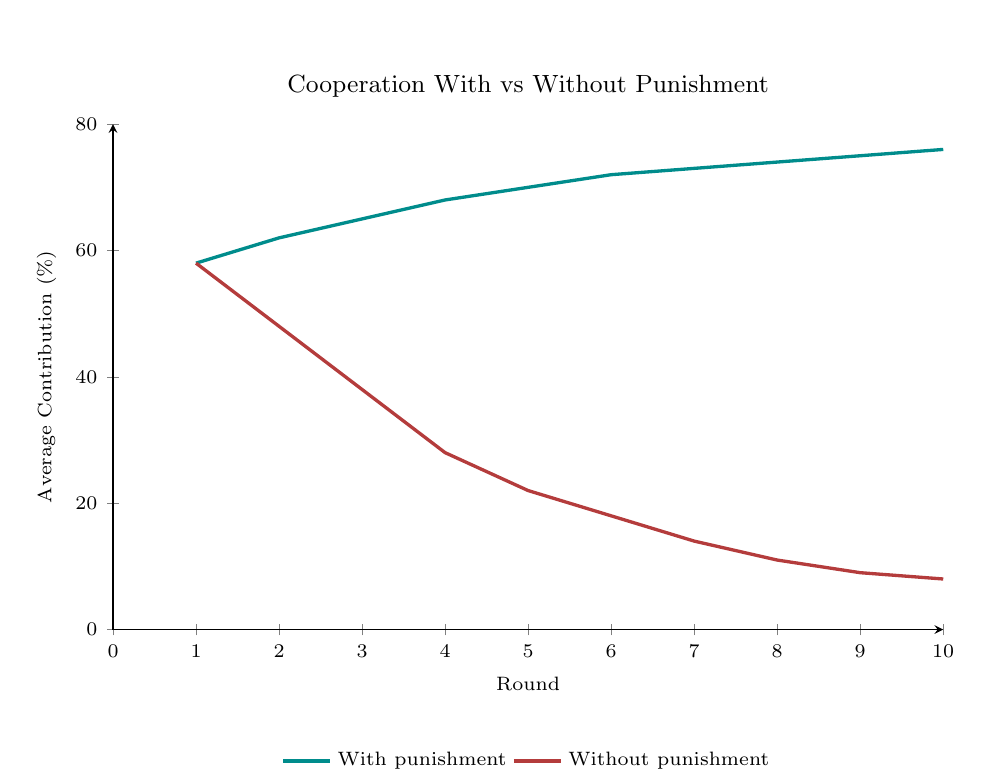
\begin{tikzpicture}
\begin{axis}[
    width=\textwidth,
    height=8cm,
    xlabel={Round},
    ylabel={Average Contribution (\%)},
    xmin=0, xmax=10,
    ymin=0, ymax=80,
    axis lines=left,
    title={Cooperation With vs Without Punishment},
    % Legend BELOW axis
    legend style={
        at={(0.5,-0.22)},
        anchor=north,
        font=\scriptsize,
        draw=none,
        fill=none,
        legend columns=2
    },
    tick label style={font=\scriptsize},
    label style={font=\scriptsize},
    title style={font=\small},
    clip=false
]

\addplot[very thick, color=beteal]
coordinates {(1,58)(2,62)(3,65)(4,68)(5,70)(6,72)(7,73)(8,74)(9,75)(10,76)};

\addplot[very thick, color=berust]
coordinates {(1,58)(2,48)(3,38)(4,28)(5,22)(6,18)(7,14)(8,11)(9,9)(10,8)};

\legend{With punishment, Without punishment}

\end{axis}
\end{tikzpicture}
\end{subfigure}

\hfill
\end{figure}


\begin{table}[H]
\centering
\small
\begin{tabularx}{\linewidth}{lY}
\toprule
 & Description \\
\midrule
\textbf{What the figure shows} & Two lines plotted against rounds (1--10). The "no punishment" line starts at approximately 58\% average contribution in round 1 and falls steadily to approximately 8\% by round 10. The "with punishment" line starts at the same level but rises across rounds, reaching approximately 76\% by round 10. The two lines cross approximately around round 3. \\
\textbf{How to interpret it} & The divergence between the two conditions, despite identical financial incentives, demonstrates that the punishment option alone --- not the threat of reputation damage or repeated interaction --- sustains cooperation. The punished free-riders adjust their behaviour; the prospect of punishment deters future free-riding; cooperation builds. This is the signature of a norm-enforcement mechanism operating through altruistic punishment. \\
\bottomrule
\end{tabularx}
\end{table}



\subsection{Reciprocity as a Foundation of Cooperation}


The public goods game evidence connects to a broader theoretical framework. Fehr and Gächter (2000) distinguish two types of reciprocity:

\textbf{Positive reciprocity:} Responding to kind actions with kindness. In the trust game, trustees return money because investors trusted them. In gift exchange experiments, workers provide effort above the minimum because employers paid above-market wages.

\textbf{Negative reciprocity:} Responding to unkind actions with punishment, even at personal cost. Responders reject unfair ultimatum offers. Players punish free-riders in public goods games. Workers reduce effort when employers offer below-market wages.

Both forms of reciprocity play a central role in maintaining social cooperation. Positive reciprocity sustains voluntary exchange and the social trust that enables economic development. Negative reciprocity enforces social norms --- including contributions to public goods, compliance with social conventions, and the norms of fairness that make market exchange possible.

The coexistence of a significant minority of self-interested agents with a majority of reciprocal and inequality-averse agents has important implications for institutional design. In a homogeneous population of purely self-interested agents, no cooperation can be sustained in one-shot public goods games. But in a heterogeneous population where even a fraction of agents are willing to punish free-riding, cooperation can be sustained --- because the credible threat of punishment by the reciprocal types deters the self-interested types from free-riding.

\medskip


\section{Models of Giving: Altruism, Warm Glow, and Impure Altruism}



\subsection{Pure Altruism}


Under pure altruism, agent $i$ cares directly about agent $j$'s utility or consumption:

$$U_i = u_i(x_i) + \theta_i \cdot u_j(x_j)$$

where $\theta_i \geq 0$ is the weight on $j$'s utility. When $\theta_i = 0$, this reduces to pure self-interest. When $\theta_i > 0$, agent $i$ is a genuine altruist --- they value $j$'s wellbeing as if it were partly their own.

Pure altruism generates clean predictions: giving increases when $j$'s need is greater; any source of income for $j$ substitutes for giving from $i$ (perfect crowding out); the identity of the recipient matters only through their utility, not through any psychological salience.


\subsection{Warm Glow and Impure Altruism}


Andreoni (1989, 1990) proposed the \textbf{warm glow} model: agents receive a private psychological reward from the \textit{act} of giving, independent of the recipient's total utility:

$$U_i = u_i(x_i) + w(g_i)$$

where $g_i$ is the amount agent $i$ gives and $w(\cdot)$ is a warm glow function (increasing, concave). The key distinction from pure altruism: the warm glow depends on $g_i$ (what I gave), not on the recipient's total income (which includes what anyone else gave).

\textbf{Impure altruism} combines both motives:

$$U_i = u_i(x_i) + \theta_i \cdot u_j(x_j) + w(g_i)$$

The warm glow component has several implications:
\begin{itemize}
\item Giving is not perfectly substitutable with others' giving --- even if the government fully provides a public good, individuals may still give for the warm glow.
\item The identifiable victim effect: people give more to a named, identified beneficiary than to an equal statistical number of anonymous beneficiaries, because the identified individual triggers stronger warm glow.
\item The donor's choice: people often prefer to direct their giving to visible, emotionally engaging causes rather than to the most cost-effective interventions --- because warm glow is generated by the act and its visibility, not by the abstract impact.
\end{itemize}

These predictions are broadly supported by the empirical evidence on charitable giving, blood donation, and voluntarism.

\medskip


\section{Applications}



\subsection{Efficiency Wages and Gift Exchange in Labour Markets}


One of the most important applications of social preference theory to economics is the explanation of \textbf{efficiency wages} --- the tendency of firms to pay wages above the market-clearing level, even when there is an excess supply of labour.

The standard explanation for efficiency wages is strategic: paying above-market wages reduces employee turnover, attracts higher-quality workers, and gives workers an incentive to avoid shirking (since they would lose the wage premium if caught). These are rational, self-interest-based explanations.

Akerlof (1982) proposed a complementary, social-preference-based explanation: \textbf{gift exchange}. Workers who receive wages above the minimum perceive the high wage as a \textit{gift} from the employer --- a signal of good faith and generous treatment. In response, workers \textit{reciprocate} with effort above the contractually required minimum. The exchange is gift-like because neither party is legally obligated to provide more than the minimum --- the high wage and the high effort are both voluntary expressions of positive reciprocity.

\begin{researchbox}
\textbf{Research Study: Gift Exchange in Experimental Labour Markets}\\[4pt]

\textbf{Researchers:} Ernst Fehr, Georg Kirchsteiger, and Arno Riedl\\[4pt]
\textbf{Year:} 1993\\[4pt]
\textbf{Research Question:} Do workers provide higher effort in response to higher wages, even in anonymous one-shot interactions where reputation effects are absent?\\[4pt]
\textbf{Method:} The researchers created an experimental "labour market" in which "firms" (subjects) posted wage offers and "workers" (subjects) chose effort levels after accepting a wage. The key features: (a) interactions were fully anonymous, (b) each firm-worker pair interacted only once, and (c) effort was individually chosen with no possibility of monitoring or punishment. The experiment directly tested whether the wage-effort relationship could survive the removal of all strategic motives.\\[4pt]
\textbf{Results:} Higher wages systematically produced higher effort --- workers who received higher wages chose to work harder, even though doing so provided no strategic benefit (no reputation to build, no punishment to avoid). The wage-effort relationship was positive, statistically robust, and economically significant.\\[4pt]
\textbf{Economic Interpretation:} The finding demonstrates that gift exchange operates as a genuine motivational force in labour markets, independent of strategic considerations. Workers who receive fair or generous treatment reciprocate with cooperative behaviour. This has implications for wage-setting: in labour markets with social preferences, competitive wage cuts may reduce productivity enough to make them unprofitable, helping to explain wage stickiness.\\[4pt]
\textbf{Behavioural Insight:} The experiment isolates pure reciprocity: the only possible explanation for positive wage-effort correlation in one-shot, anonymous interactions is that workers have intrinsic preferences for reciprocating kindness. This matches Akerlof's gift exchange theory and provides direct evidence for the social preference mechanisms it invokes.\\[4pt]
\end{researchbox}

\textbf{Implications for management.} The gift exchange evidence implies that wage policy has motivational consequences beyond the incentive effects analysed by standard economics. Workers who perceive their wages as fair or generous will provide more discretionary effort --- effort that cannot be contracted for --- than workers who perceive their wages as inadequate. This has practical consequences:

\begin{itemize}
\item Unexplained wage cuts can trigger effort reductions that more than offset the labour cost savings.
\item Transparent pay structures --- where workers can verify that their wages are fair relative to their contribution and market rates --- build reciprocal motivations that increase productivity.
\item Pay confidentiality policies, which prevent workers from knowing what colleagues earn, may backfire if workers believe (correctly or not) that pay is inequitably distributed.
\end{itemize}


\subsection{Wage Rigidity and Nominal Downward Stickiness}


Chapter 4 introduced nominal wage rigidity as an application of reference dependence and loss aversion. Social preferences provide an additional, independent explanation. Workers who have developed positive reciprocal relationships with their employers based on fair wages will experience a nominal wage cut as a violation of the implicit reciprocal norm --- not merely as a financial loss. The response to this norm violation includes:

\begin{itemize}
\item Reduced effort (withdrawal of discretionary input above the contractual minimum)
\item Reduced cooperation with management initiatives
\item Increased turnover (exit) and absenteeism
\item Collective resistance through unions or informal norms
\end{itemize}

Akerlof, Dickens, and Perry (1996) documented the empirical consequence: nominal wage cuts are extraordinarily rare even in recessions when standard theory predicts they should occur. Employers adjust to adverse economic conditions through layoffs, hours reductions, and real wage erosion through inflation --- rather than nominal cuts --- because nominal cuts trigger the reciprocal withdrawal response that makes them costly.

This mechanism operates in addition to (and independently of) the loss aversion mechanism studied in Chapter 4. Together, the two mechanisms generate a very strong prediction of downward nominal wage rigidity, which is one of the most robust and economically significant findings in macroeconomics.


\subsection{Inequality, Morale, and Firm Performance}


The Fehr-Schmidt model implies that within-firm inequality in pay can reduce worker utility and potentially reduce effort among low-paid workers who experience disadvantageous inequality aversion. Card and colleagues (2012) tested this prediction directly in a field experiment with employees at the University of California.

In 2008, the California Supreme Court ruled that UC's employee pay data must be made public. Card et al. used this event as a natural experiment: they informed a random subset of employees about the university's new pay transparency website, then surveyed workers about their job satisfaction and job search behaviour.

Workers who discovered they were paid below the median for their department and occupation reported significantly lower job satisfaction and significantly higher intentions to search for new jobs --- consistent with strong disadvantageous inequality aversion. Interestingly, above-median earners showed essentially no change in satisfaction or job search behaviour --- consistent with the Fehr-Schmidt model, in which advantageous inequality (being above others) generates less strong preference effects than disadvantageous inequality.

This finding has direct policy implications for corporate pay transparency. Advocates of pay transparency argue that it reduces discrimination and promotes fairness. Critics worry it will reduce morale among those who discover they earn less than peers. The Card et al. evidence suggests both concerns are partly valid: transparency increases dissatisfaction among below-median earners but does not significantly benefit above-median earners.


\subsection{Social Norms, Trust, and Corruption}


The trust game and the Fisman-Miguel (2007) study of UN diplomatic parking violations converge on a striking conclusion: social norms of honesty and civic behaviour are \textbf{internalised}, not merely imposed externally by legal systems. People from high-trust, low-corruption societies comply with civic norms even when there is no legal enforcement --- because they genuinely believe in and value those norms. People from low-trust, high-corruption societies violate norms even when the personal cost of violation is negligible --- because they do not internalise those norms as binding.

\begin{researchbox}
\textbf{Research Study: Corruption Norms and Diplomatic Immunity --- A Natural Experiment}\\[4pt]

\textbf{Researchers:} Raymond Fisman and Edward Miguel\\[4pt]
\textbf{Year:} 2007\\[4pt]
\textbf{Research Question:} Do cultural norms of corruption persist when formal legal enforcement is removed?\\[4pt]
\textbf{Method:} Before November 2002, United Nations diplomats in New York City had full diplomatic immunity from enforcement of parking violations --- they could park illegally with no legal consequence whatsoever. After 2002, the US government began withholding aid from countries whose diplomats had unpaid violations. Fisman and Miguel used the pre-2002 period as a natural experiment: any variation in parking violations across countries reflected purely the internalised norms of the diplomatic staff, since legal incentives were identical (zero) for all.\\[4pt]
\textbf{Results:} The variation was enormous and systematic. Diplomats from Scandinavian countries (Norway, Sweden, Denmark) had near-zero violations. Diplomats from Canada had near-zero violations. Diplomats from many developing economies with high corruption scores accumulated hundreds of violations per diplomat. Critically, the number of violations per diplomat was strongly positively correlated with Transparency International's Corruption Perceptions Index for the diplomat's home country.\\[4pt]
\textbf{Economic Interpretation:} When legal enforcement is removed, the only remaining determinant of compliance is internalised norms. The strong correlation between home-country corruption and parking violations demonstrates that corruption is not merely a response to weak enforcement --- it reflects genuinely different internalised norms about civic obligation and respect for rules. People from low-corruption cultures comply because they believe in the rules; people from high-corruption cultures violate them because they do not.\\[4pt]
\textbf{Behavioural Insight:} Social norms are not merely external constraints. They are internalised standards of behaviour that people carry with them across contexts. This has implications for anti-corruption policy: legal reforms that increase enforcement may reduce corruption temporarily, but lasting change requires norm transformation --- which is much harder to achieve and much slower to materialise than changes in enforcement.\\[4pt]
\end{researchbox}

\textbf{Policy implications.} The Fisman-Miguel study suggests that anti-corruption efforts should not focus exclusively on improving legal enforcement and increasing penalties. While these measures help in the short run, sustainable reductions in corruption require building cultures of civic trust and internalised norms --- through education, leadership examples, institutional designs that make norm compliance visible and socially rewarded, and gradual reduction in contexts where corruption is expected.

Canada's relatively low level of corruption (typically ranking among the top 15--20 countries globally on Transparency International's index, with a 2023 score of 76/100) reflects decades of institutional building, professional cultures of public service, and civic norms that treat public resources as genuinely distinct from private interests.


\subsection{Corporate Social Responsibility and Stakeholder Preferences}


Social preference theory also helps explain the widespread demand for \textbf{corporate social responsibility (CSR)} --- firm behaviour that goes beyond legal requirements to consider the welfare of employees, communities, and the environment. Standard economics predicts that in competitive markets, firms should single-mindedly maximise shareholder value; any diversion of resources to social objectives reduces profits and should be punished by capital markets.

In practice, firms devote substantial resources to CSR --- and some evidence suggests this is economically rational:

\begin{itemize}
\item \textbf{Consumer demand:} Consumers with social preferences are willing to pay premiums for fair-trade, environmentally friendly, or ethically sourced products. Surveys consistently show that a significant fraction of consumers (approximately 30--50\%) say they would pay more for products from socially responsible firms.
\item \textbf{Worker motivation:} Workers with social preferences may accept lower wages to work for firms with good social or environmental records --- effectively subsidising CSR through the labour market.
\item \textbf{Investor preferences:} The growth of ESG (Environmental, Social, Governance) investing suggests that a substantial fraction of investors have preferences over the social impact of their investments beyond returns.
\end{itemize}

Whether CSR is primarily driven by genuine social preferences or by strategic calculation (building reputation, managing regulatory risk, attracting talent) remains debated. The social preference framework suggests both are operative: some CSR reflects genuine altruistic preferences among owners, managers, and workers; some reflects strategic calculation in markets where consumers and employees have social preferences that create financial returns to social behaviour.

\medskip


\section{Cultural Variation and the Limits of Social Preference Models}



\subsection{What Varies and What Does Not}


The cross-cultural evidence from Henrich and colleagues and from studies of social trust establishes two conclusions that seem, at first, contradictory:

\begin{enumerate}
\item \textbf{Universal:} No human society studied shows behaviour consistent with pure self-interest. Social preferences --- in some form --- are a universal feature of human psychology.
\end{enumerate}

\begin{enumerate}
\item \textbf{Variable:} The specific form, strength, and context-dependence of social preferences varies substantially across cultures, economic systems, and institutions.
\end{enumerate}

Reconciling these findings requires attention to the distinction between the \textit{capacity} for social preferences (which appears universal) and their \textit{expression} (which is culturally shaped). All humans appear to have the psychological capacity for fairness concern, reciprocity, and altruism --- evolved features of the human mind. But how strongly these preferences operate, in which contexts they apply, toward whom they extend, and what they consider "fair" is shaped by cultural norms, economic institutions, and lived experience.


\subsection{In-Group versus Out-Group Social Preferences}


One of the most robust cross-cultural findings is that social preferences are typically stronger toward in-group members (people from one's own community, ethnic group, or social network) than toward out-group members (strangers, members of other groups). Bernhard, Fischbacher, and Fehr (2006) documented this directly: in a three-player punishment game in Papua New Guinea, subjects showed much stronger punishment of in-group free-riders than out-group free-riders, and in some cases did not punish out-group free-riders at all.

This in-group/out-group distinction has important economic implications:

\begin{itemize}
\item \textbf{Migration and integration:} Trust and cooperation may be lower in ethnically diverse communities, not because diversity inherently reduces social preferences but because social preferences extend less readily to out-group members. Putnam (2007) found evidence of this "diversity penalty" in US communities, though the finding is contested and appears to depend heavily on the history of intergroup contact.
\item \textbf{Corruption and tribalism:} Corruption often operates through in-group networks: officials use public resources to benefit their family, ethnic group, or social network --- an expression of in-group social preferences that violates civic norms of impartial treatment.
\item \textbf{Trade and globalisation:} Economic exchange between culturally different groups requires mechanisms --- contracts, international law, trade organisations --- that substitute for the social trust that operates within groups.
\end{itemize}

\newpage


\section*{Critical Thinking Questions}
\addcontentsline{toc}{section}{Critical Thinking Questions}

\subsection{Conceptual Questions}

\begin{enumerate}
\item The ultimatum game shows that people reject positive offers of money. A standard economist might argue this is irrational --- \$5 is better than \$0. A behavioural economist argues it reflects a social preference for fairness. Which view is more defensible? Is rejecting an unfair offer ever \textit{rational} in any economically meaningful sense?

\item The dictator game shows that 64\% of Dictators give some money to the recipient, even without any strategic incentive to do so. Three possible explanations are offered: pure altruism, warm glow, and social image concerns. Design an experiment that would distinguish between these three explanations.

\item The Fehr-Schmidt model assumes that agents care about the distribution of payoffs, not about the intentions behind those payoffs. Blount (1995) showed that people respond differently to the same offer depending on whether it was generated by a human or a random device. What does this imply about the adequacy of outcome-based models? How would you modify the Fehr-Schmidt utility function to incorporate intentionality?

\item Altruistic punishment --- paying a personal cost to punish a norm violator who will never interact with you again --- is hard to explain under pure self-interest. Propose an evolutionary argument for why altruistic punishment might have emerged as an adaptive trait. What selection pressures would favour it?


\item The trust game shows that investors (A) send significant amounts to trustees (B) despite the rational prediction that they should send nothing. Two explanations are offered: altruism (A cares about B's welfare) and trust (A expects B to reciprocate). Can you design an experiment that cleanly separates these two motives?

\item The Fehr-Schmidt model predicts that disadvantageous inequality ($\alpha$) generates stronger disutility than advantageous inequality ($\beta$). What is the intuition for this asymmetry? Is it consistent with evolutionary arguments about cooperation? Can you think of exceptions?

\item Pure altruism predicts that government provision of a public good should perfectly crowd out private giving. The empirical evidence shows incomplete crowding out. What does this imply about the dominant motive for charitable giving? What are the policy implications for how governments should design co-funding arrangements with charities?

\item Cross-cultural ultimatum game studies show that no society behaves according to the Nash prediction, yet there is enormous variation across societies. What does this tell us about the relative importance of universal human psychology versus cultural institutions in determining economic behaviour?

\item The Fisman-Miguel parking study shows that social norms persist even when legal enforcement is removed. But it also shows enormous variation across countries --- some diplomats violate norms and others do not. What determines which norms get internalised and which remain purely externally enforced? What can governments do to facilitate internalisation of civic norms?

\item The in-group/out-group distinction in social preferences suggests that people cooperate more within their social group than across groups. Does this imply that market integration and globalisation --- which require cooperation with strangers --- erode social preferences, or does it suggest that exposure to diverse others can expand the scope of social preferences?
\end{enumerate}


\subsection{Application Questions}


\begin{enumerate}
\item A firm is considering two wage-setting strategies. Strategy A: pay all workers \$60,000/year with no pay transparency. Strategy B: pay workers \$55,000 on average but with complete pay transparency and clear, merit-based justifications for pay differences. Using the Fehr-Schmidt model and the gift exchange evidence, predict which strategy will generate higher effort and lower turnover. What additional information would you need to make a definitive recommendation?

\item A school district is designing a teacher pay system. Option A: all teachers receive the same salary regardless of performance. Option B: top-performing teachers receive a 25\% bonus. Using the evidence on inequality aversion and altruistic punishment, what concerns would you raise about Option B? Are these concerns sufficient to recommend Option A?

\item The Canadian Red Cross relies heavily on voluntary blood donation. Using the distinctions among pure altruism, warm glow, and social image, design a donation campaign that maximises donation rates. Specifically: should the campaign emphasise recipients' need, the personal act of donating, or social recognition of donors?
\newpage
\item A government is designing a tax compliance enforcement strategy. One approach emphasises audits and penalties (legal enforcement). Another emphasises social norms messaging --- "Most Canadians pay their full taxes" (norm activation). Using the Fisman-Miguel evidence and social preference theory, predict the relative effectiveness of each approach. Under what conditions would each work best?

\item A startup CEO wants to build a "high-trust" company culture. Based on the trust game evidence and the gift exchange research, describe five specific management practices they should implement, explaining the behavioural mechanism through which each builds trust and reciprocal effort.

\item A provincial government is considering publishing the salaries of all public servants. Advocates argue this promotes fairness and reduces discrimination. Critics argue it will reduce morale among lower-paid employees. Using the Card et al. (2012) evidence, assess both sides. What additional design features --- beyond simple publication --- would you recommend to maximise the benefits and minimise the costs?

\item Imagine you are designing the rules for a neighbourhood association that maintains a shared community garden. Each household is asked to volunteer 2 hours per month. No enforcement mechanism currently exists. Using the public goods game evidence, predict what will happen to participation over time. Design a minimum intervention that would sustain cooperation without requiring significant monitoring costs.


\item A large Canadian bank is evaluating its CSR programme --- donations to community organisations, environmental initiatives, and fair-trade supplier practices. The CFO argues these activities cost \$50 million per year and should be cut because they don't directly increase profits. The CEO argues they are economically valuable. Construct the CEO's argument using social preference theory, citing specific mechanisms (consumer preferences, worker motivation, investor preferences) and supporting evidence.

\item A country is experiencing a wave of public corruption. The government instals a new anti-corruption monitoring system with significant penalties. Corruption falls by 30\% immediately. Five years later, after the monitoring system is removed due to budget cuts, corruption returns to its original level within two years. Using the Fisman-Miguel framework and social preference theory, diagnose what went wrong and recommend a long-term approach.
\newpage
\item An online platform is experiencing a "tragedy of the commons" --- users are leaving increasingly poor-quality content because the platforms' rating systems are gamed by free-riders. Using the altruistic punishment evidence, design a moderation system that harnesses users' willingness to punish norm violators. What features would maximise voluntary participation in moderation?
\end{enumerate}


\subsection{Discussion Questions}


\begin{enumerate}
\item Rejecting an unfair ultimatum offer sacrifices money to "send a message." But in a one-shot anonymous game, there is no one to receive the message --- the Proposer will never know you rejected, and you will never interact again. What, then, is the functional purpose of rejection? Does it matter that the rejection has no audience?

\item The Fehr-Schmidt model and the Bolton-Ockenfels ERC model both explain ultimatum game behaviour, but with different underlying motivations. Does it matter which model is correct? If both fit the experimental data equally well, on what grounds would you choose between them? What novel experiments would discriminate between them?

\item "Social preferences are fine for small-scale interactions --- family, neighbours, colleagues. But in large anonymous markets, they are irrelevant. Markets select for self-interest." Evaluate this claim. What evidence suggests social preferences operate in large, anonymous market settings? What evidence supports the claim?

\item The Henrich et al. cross-cultural study found that greater market integration (exposure to market exchange) was positively associated with higher ultimatum offers and stronger rejection of unfair treatment. This is counterintuitive --- markets are usually thought to promote self-interest. How would you explain this finding? What mechanism links market exposure to fairer social preferences?

\item Altruistic punishment is costly to the punisher and the punished but benefits third parties (by deterring future free-riding). Does this mean that those who punish free-riders are themselves acting altruistically toward the group --- even when their motivation is anger and moral indignation? Can anger and altruism coexist as motivations for the same act?

\item Warm glow altruism implies that people give to charities partly for the psychological reward of giving, not primarily for the recipient's benefit. Does this mean charitable giving is "selfish"? Does it matter whether the motivation is warm glow versus pure altruism, as long as the recipient receives the donation?

\item The gift exchange evidence shows that workers provide higher effort in response to higher wages, even in one-shot anonymous interactions. But field evidence on worker motivation is more mixed --- many studies find that performance pay and monitoring are more effective than high base wages in increasing effort. How do you reconcile the laboratory and field evidence? When does gift exchange motivate behaviour, and when does it not?

\item The Fisman-Miguel study shows that diplomats from high-corruption countries park illegally more often even when legal enforcement is zero. But this could reflect different subjective beliefs about whether parking violations are actually harmful, rather than different norms of civic compliance. How would you redesign the study to test whether the violation reflects norm differences or belief differences?

\item Social preferences include altruism, inequality aversion, and reciprocity. In real economic settings, all three may operate simultaneously and may sometimes conflict. Give an example of an economic situation in which altruism, inequality aversion, and reciprocity generate contradictory predictions --- and explain how you would determine which motivation dominates.

\item "Teaching economics has the side effect of making students more selfish." Some studies suggest that economics students contribute less to public goods, are more likely to defect in prisoner's dilemma games, and make lower ultimatum offers than non-economics students. If this is true, what does it imply about the effects of teaching standard economics? Does teaching behavioural economics correct the effect? Should it?
\end{enumerate}

\newpage


\section*{Chapter Summary}
\addcontentsline{toc}{section}{Chapter Summary}


This chapter has developed the theory and evidence for social preferences --- motivations that extend beyond pure self-interest to include genuine concern for others' outcomes, fairness, reciprocity, and social norms.

\textbf{The failure of pure self-interest.} In every major experimental paradigm --- ultimatum, dictator, trust, and public goods games --- behaviour systematically and substantially departs from the Nash equilibrium prediction under pure self-interest. Mean ultimatum offers are approximately 40--44\% of the pie; 40--60\% of Responders reject offers below 20\%. Mean dictator game giving is approximately 28\% even with no strategic motive. Trust game investors send approximately 50\% of their endowment and receive approximately 37\% of the tripled amount back. Public goods contributions start at 40--60\% and decline only when no punishment mechanism exists.

\textbf{The ultimatum game.} Proposers offer more than self-interest requires; Responders reject positive offers that are perceived as unfair. The pattern is robust to high stakes (Slonim and Roth, 1998; Cameron, 1999) and cross-cultural (Henrich et al., 2001, 2004). No society studied shows behaviour close to the Nash prediction; all show social preferences of some kind. Market integration is positively associated with fairer offers.

\textbf{The dictator game.} Giving by Dictators who face no strategic considerations reveals genuine social preferences. The distribution is bimodal: approximately 36\% give nothing (consistent with self-interest), approximately 17\% give exactly half, with the remainder giving intermediate amounts. Giving is affected by anonymity (image concerns), earned endowments (legitimacy of the distribution), and recipient identity (warm glow for salient causes).

\textbf{The trust game.} Trust and trustworthiness coexist in economic interactions. Investors send significant amounts despite the rational prediction of zero; trustees return positive amounts despite no obligation to do so. Cox (2004) shows that both altruism and reciprocity motivate trustee returns approximately equally. Social trust at the country level predicts economic growth (Knack and Keefer, 1997).

\textbf{The Fehr-Schmidt model.} Inequality aversion --- disutility from both disadvantageous inequality (envy, parameter $\alpha$) and advantageous inequality (guilt, parameter $\beta$) --- provides a tractable formal model with good empirical fit. The minimum acceptance threshold in the ultimatum game equals $\alpha/(1+2\alpha)$, generating predictions consistent with observed rejection patterns. The model's limitation is its purely outcome-based structure, which misses intentionality effects and reciprocity.

\textbf{Altruistic punishment.} People pay personal costs to punish norm violators even in one-shot interactions with no reputational benefit. Fehr and Gächter (2002) showed that a punishment option raises public goods contributions from near-zero to over 70\%, while no-punishment contributions decline to near-zero. Altruistic punishment is the mechanism through which social norms are enforced in the absence of legal coercion.

\textbf{Applications.} Social preferences generate economically important phenomena: efficiency wages and gift exchange in labour markets (Akerlof, 1982; Fehr, Kirchsteiger, and Riedl, 1993); wage rigidity through norm violation aversion; pay transparency effects on morale (Card et al., 2012); persistent corruption norms internalised from home countries (Fisman and Miguel, 2007); and CSR demand from consumers and workers with social preferences.
\newpage


\section*{Glossary}
\addcontentsline{toc}{section}{Glossary}


\textbf{Altruism (Pure).} A social preference in which agent $i$ cares directly about agent $j$'s welfare or utility: $U_i = u_i(x_i) + \theta_i u_j(x_j)$, with $\theta_i > 0$. Giving from pure altruism is perfectly substitutable with giving from other sources --- the altruist cares about the recipient's total welfare, not about being the source. \textit{Distinction from warm glow:} Pure altruists reduce giving when others give more (crowding out); warm glow givers maintain giving even when others give.

\textbf{Altruistic Punishment.} The disposition to punish norm violators at personal cost, even in one-shot interactions where there is no future material benefit to the punisher. The key experimental finding of Fehr and Gächter (2002): subjects pay 1 unit to reduce a free-rider's earnings by 3 units, despite no future interaction. \textit{Why it matters:} Provides the enforcement mechanism for social norms in the absence of legal coercion; explains how cooperation is sustained in large groups of genetically unrelated individuals.

\textbf{Conditional Cooperation.} The tendency to contribute to public goods when others contribute, and reduce contributions when others free-ride. Most subjects in public goods games are conditional cooperators rather than either unconditional contributors or unconditional free-riders. \textit{Why it matters:} Explains the characteristic decline in cooperation over time in public goods experiments without punishment: conditional cooperators respond to observed free-riding by reducing their own contributions.

\textbf{Dictator Game.} An experimental design in which one player (the Dictator) unilaterally divides an endowment between themselves and a passive recipient who must accept whatever is offered. Any giving by the Dictator is a pure expression of social preferences --- altruism, inequality aversion, or warm glow --- with no strategic motive. \textit{Typical result:} Mean giving $\approx$ 28\% (Engel, 2011 meta-analysis); 36\% give \$0, 17\% give 50\%.

\textbf{Efficiency Wages.} Wages paid above the market-clearing level, motivated partly by the desire to generate gift exchange: workers who receive above-market wages reciprocate with above-minimum effort. Akerlof (1982) formalised this as labour market gift exchange. Explains why wages do not fall to clear labour markets in recessions.

\textbf{Fehr-Schmidt Model.} A model of inequality aversion in which agent $i$'s utility is:
\[
U_i = x_i - \alpha_i \max(x_j - x_i, 0) - \beta_i \max(x_i - x_j, 0).
\]

Parameter $\alpha_i$ captures disutility from disadvantageous inequality (envy); parameter $\beta_i$ captures disutility from advantageous inequality (guilt).

Constraints: $\alpha_i \geq \beta_i \geq 0$, $\beta_i < 1$.

\textit{Calibrated values:} $\bar{\alpha} \approx 0.5$--$1.0$, $\bar{\beta} \approx 0.2$--$0.4$.

\textit{Why it matters:} The most widely used formal model of social preferences; it generates predictions for ultimatum, dictator, and public goods game behaviour across heterogeneous populations.

\textbf{Free-Rider Problem.} The incentive for individuals to benefit from a public good without contributing to its provision, since the good is non-excludable. In a pure self-interest model, rational agents always free-ride; the equilibrium is zero provision despite positive social value. Social preferences --- altruism, inequality aversion, reciprocity --- and altruistic punishment mitigate the free-rider problem.

\textbf{Gift Exchange.} The reciprocal pattern in labour markets and social interactions in which above-market wages (the "gift" from employer to worker) are reciprocated with above-minimum effort (the "gift" from worker to employer). A key mechanism through which positive reciprocity operates in economic settings.

\textbf{Inequality Aversion.} The disutility that agents experience from unequal distributions of payoffs --- whether they are on the disadvantaged or advantaged side of the inequality. Formalised by Fehr and Schmidt (1999) through parameters for disadvantageous inequality aversion ($\alpha$) and advantageous inequality aversion ($\beta$).

\textbf{In-Group/Out-Group Distinction.} The tendency for social preferences --- trust, reciprocity, altruism, and punishment --- to operate more strongly toward members of one's own social group (in-group) than toward members of other groups (out-group). Has implications for cooperation in diverse societies and for the scope of markets that can be sustained without formal enforcement.

\textbf{Public Goods Game.} An experimental paradigm in which players simultaneously decide how much to contribute to a group pot that is multiplied and divided equally among all players. The Nash equilibrium under self-interest is zero contribution; empirical results show substantial initial contributions (40--60\%) that decline over time without a punishment mechanism.

\textbf{Reciprocity.} The disposition to respond to kind actions with kindness (positive reciprocity) and to unkind actions with punishment (negative reciprocity), even at personal cost and even in one-shot interactions where reputation effects are absent. Reciprocity is intention-based: the response depends on perceived intentions, not just payoff outcomes.

\textbf{Social Capital.} The productive capacity generated by social trust, cooperative norms, and networks of reciprocal relationships within a community or society. Higher social capital reduces the transaction costs of economic exchange and enables complex specialisation. Knack and Keefer (1997) estimate that a one-standard-deviation increase in social trust increases annual GDP growth by approximately 0.5 percentage points.

\textbf{Social Preferences.} Genuine motivations that extend beyond own-payoff maximisation to include concern for others' outcomes, fairness, and social norms. Include altruism, inequality aversion, reciprocity, and warm glow. Documented across cultures, stake sizes, and institutional settings; cannot be explained by strategic motives (reputation, repeated interaction) because they persist in one-shot anonymous interactions.

\textbf{Trust Game.} An experimental paradigm introduced by Berg, Dickhaut, and McCabe (1995) in which Player A can send money to Player B (which triples in transit), and B can voluntarily return any amount. Under backward induction with self-interest, the Nash equilibrium is: A sends \$0. Typical result: A sends $\approx$50\%, B returns $\approx$37\% of the tripled amount.

\textbf{Ultimatum Game.} An experimental paradigm in which a Proposer divides a pie and a Responder either accepts (both get the proposed amounts) or rejects (both get nothing). Under self-interest, the unique subgame perfect Nash equilibrium is: Proposer offers \$0.01, Responder accepts. Typical result: mean offers $\approx$ 40--44\%; offers below 20\% rejected by 40--60\% of Responders.

\textbf{Warm Glow Altruism.} The psychological reward received by the giver from the \textit{act} of giving, independent of the recipient's total welfare. Formalised by Andreoni (1989, 1990): $U_i = u_i(x_i) + w(g_i)$ where $g_i$ is the amount given. Unlike pure altruism, warm glow giving is not perfectly substituted by others' giving --- the psychological reward depends on the agent's own action. \textit{Evidence:} Incomplete crowding out of private by public provision; the identifiable victim effect; preferences for directing giving to salient causes over statistically equivalent but less visible needs.

\medskip


\section*{References}
\addcontentsline{toc}{section}{References}


Akerlof, G. A. (1982). Labor contracts as partial gift exchange. \textit{Quarterly Journal of Economics}, 97(4), 543--569.

Akerlof, G. A., Dickens, W. T., \& Perry, G. L. (1996). The macroeconomics of low inflation. \textit{Brookings Papers on Economic Activity}, 1, 1--76.

Andreoni, J. (1989). Giving with impure altruism: Applications to charity and Ricardian equivalence. \textit{Journal of Political Economy}, 97(6), 1447--1458.

Andreoni, J. (1990). Impure altruism and donations to public goods: A theory of warm-glow giving. \textit{Economic Journal}, 100(401), 464--477.

Andreoni, J. (1993). An experimental test of the public-goods crowding-out hypothesis. \textit{American Economic Review}, 83(5), 1317--1327.

Andreoni, J., \& Bernheim, B. D. (2009). Social image and the 50--50 norm: A theoretical and experimental analysis of audience effects. \textit{Econometrica}, 77(5), 1607--1636.

Becker, G. S. (1974). A theory of social interactions. \textit{Journal of Political Economy}, 82(6), 1063--1093.

Berg, J., Dickhaut, J., \& McCabe, K. (1995). Trust, reciprocity, and social history. \textit{Games and Economic Behavior}, 10(1), 122--142.

Bernhard, H., Fischbacher, U., \& Fehr, E. (2006). Parochial altruism in humans. \textit{Nature}, 442(7105), 912--915.

Blount, S. (1995). When social outcomes aren't fair: The effect of causal attributions on preferences. \textit{Organizational Behavior and Human Decision Processes}, 63(2), 131--144.

Bolton, G. E., \& Ockenfels, A. (2000). ERC: A theory of equity, reciprocity, and competition. \textit{American Economic Review}, 90(1), 166--193.

Cameron, L. A. (1999). Raising the stakes in the ultimatum game: Experimental evidence from Indonesia. \textit{Economic Inquiry}, 37(1), 47--59.

Card, D., Mas, A., Moretti, E., \& Saez, E. (2012). Inequality at work: The effect of peer salaries on job satisfaction. \textit{American Economic Review}, 102(6), 2981--3003.

Cox, J. C. (2004). How to identify trust and reciprocity. \textit{Games and Economic Behavior}, 46(2), 260--281.

Engel, C. (2011). Dictator games: A meta study. \textit{Experimental Economics}, 14(4), 583--610.

Fehr, E., \& Gächter, S. (2000). Cooperation and punishment in public goods experiments. \textit{American Economic Review}, 90(4), 980--994.

Fehr, E., \& Gächter, S. (2002). Altruistic punishment in humans. \textit{Nature}, 415(6868), 137--140.

Fehr, E., Kirchsteiger, G., \& Riedl, A. (1993). Does fairness prevent market clearing? An experimental investigation. \textit{Quarterly Journal of Economics}, 108(2), 437--459.

Fehr, E., \& Schmidt, K. M. (1999). A theory of fairness, competition, and cooperation. \textit{Quarterly Journal of Economics}, 114(3), 817--868.

Fisman, R., \& Miguel, E. (2007). Corruption, norms, and legal enforcement: Evidence from diplomatic parking tickets. \textit{Journal of Political Economy}, 115(6), 1020--1048.

Güth, W., Schmittberger, R., \& Schwarze, B. (1982). An experimental analysis of ultimatum bargaining. \textit{Journal of Economic Behavior and Organization}, 3(4), 367--388.

Henrich, J., Boyd, R., Bowles, S., Camerer, C., Fehr, E., Gintis, H., \& McElreath, R. (2001). In search of Homo Economicus: Behavioral experiments in 15 small-scale societies. \textit{American Economic Review}, 91(2), 73--78.

Knack, S., \& Keefer, P. (1997). Does social capital have an economic payoff? A cross-country investigation. \textit{Quarterly Journal of Economics}, 112(4), 1251--1288.

Oosterbeek, H., Sloof, R., \& van de Kuilen, G. (2004). Cultural differences in ultimatum game experiments: Evidence from a meta-analysis. \textit{Experimental Economics}, 7(2), 171--188.

Putnam, R. D. (2007). E pluribus unum: Diversity and community in the twenty-first century. \textit{Scandinavian Political Studies}, 30(2), 137--174.

Rabin, M. (1993). Incorporating fairness into game theory and economics. \textit{American Economic Review}, 83(5), 1281--1302.

Slonim, R., \& Roth, A. E. (1998). Learning in high stakes ultimatum games: An experiment in the Slovak Republic. \textit{Econometrica}, 66(3), 569--596.

Smith, A. (1759). \textit{The Theory of Moral Sentiments}. Millar.

Transparency International. (2023). \textit{Corruption Perceptions Index 2023}. Transparency International.

World Values Survey Association. (2022). \textit{World Values Survey Wave 7: 2017--2022}. JD Systems Institute.

\medskip

\textit{End of Chapter 6}

\medskip

\begin{quote}
\textbf{Looking Ahead.} Chapter 7 takes social preferences into strategic settings: game theory. We have documented that people are not purely self-interested, but classical game theory still assumes players reason to the Nash equilibrium through deep recursive logic. Chapter 7 examines the evidence against this assumption --- the beauty contest game, the centipede game, and experimental coordination games --- and introduces behavioural alternatives: level-k thinking, the cognitive hierarchy model, and quantal response equilibrium. Together with the social preferences studied in this chapter, these models form the foundation of \textbf{behavioural game theory}: a more realistic account of strategic interaction that accounts for bounded rationality and social motivations simultaneously.
\end{quote}

\end{document}
